\section{Results}
\label{sec:results}

We present results in the order of our causal chain: first establishing that orbits are geometrically large (RQ1), then probing whether NFT is invariant to them (RQ2), then testing whether canonicalization concentrates structure (RQ3), and finally auditing the structural validity of the sign-flip algorithm (RQ4). Property prediction directional results (RQ5) are presented last.

\subsection{Orbit Diameter Characterization (RQ1)}

\textbf{Both symmetry types produce geometrically large orbits.} Table~\ref{tab:orbit} summarizes orbit diameter measurements for $N=500$ oracle-constructed orbit pairs per symmetry type.

\begin{table}[h]
\centering
\caption{Orbit Diameter Statistics ($N=500$ oracle pairs per symmetry type).}
\label{tab:orbit}
\begin{tabular}{lllll}
\toprule
Symmetry & Mean cosine dist. & 95\% CI & Fraction $> 0.05$ & 95\% CI \\
\midrule
Scaling & 0.3232 & [0.3226, 0.3238] & 1.000 & [1.000, 1.000] \\
Sign-flip & 1.075 & [1.0705, 1.0789] & 1.000 & [1.000, 1.000] \\
\bottomrule
\end{tabular}
\end{table}

Scaling orbits have mean cosine distance 0.3232 --- roughly 30\% of the maximum possible cosine distance of 2.0. Sign-flip orbits are far larger, with mean cosine distance 1.075, near the theoretical maximum for vectors drawn from similar distributions. Every single oracle orbit pair (100\%, $N=2{,}500$ including all five conditions) exceeds the geometric significance threshold of 0.05 cosine distance.

\begin{figure}[t]
\centering
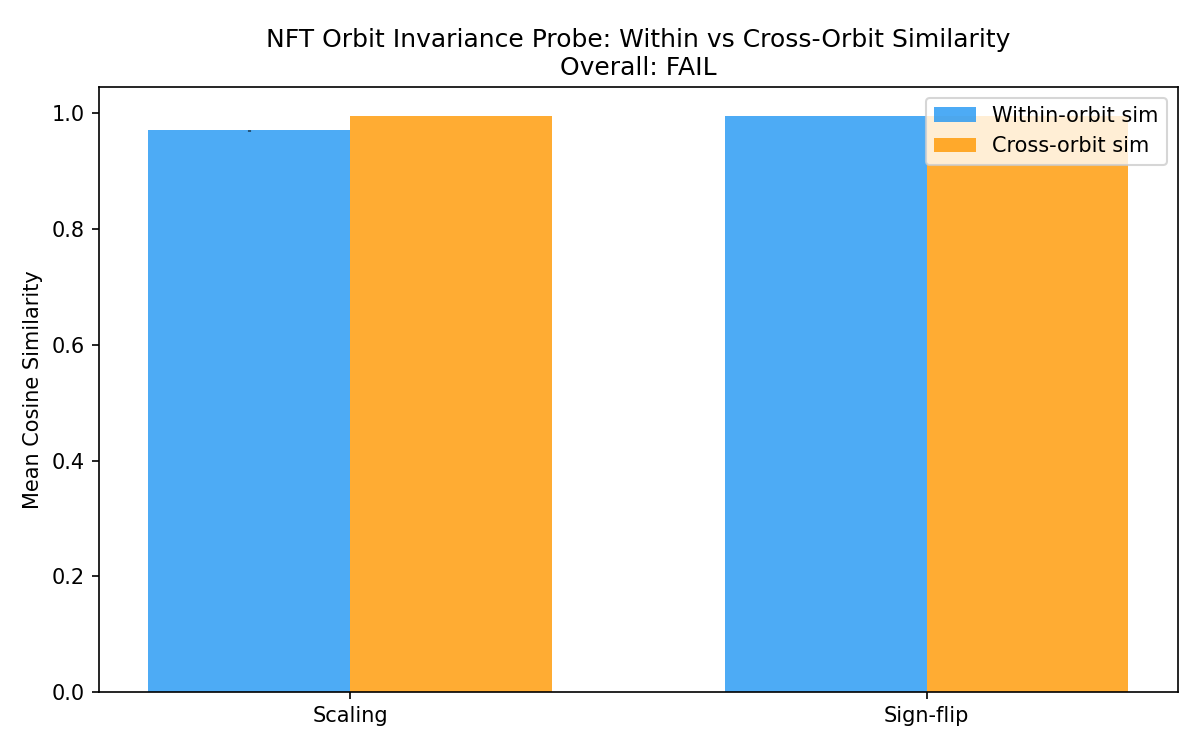
\includegraphics[width=0.48\linewidth]{figures/fig_gate_metrics.png}
\hfill
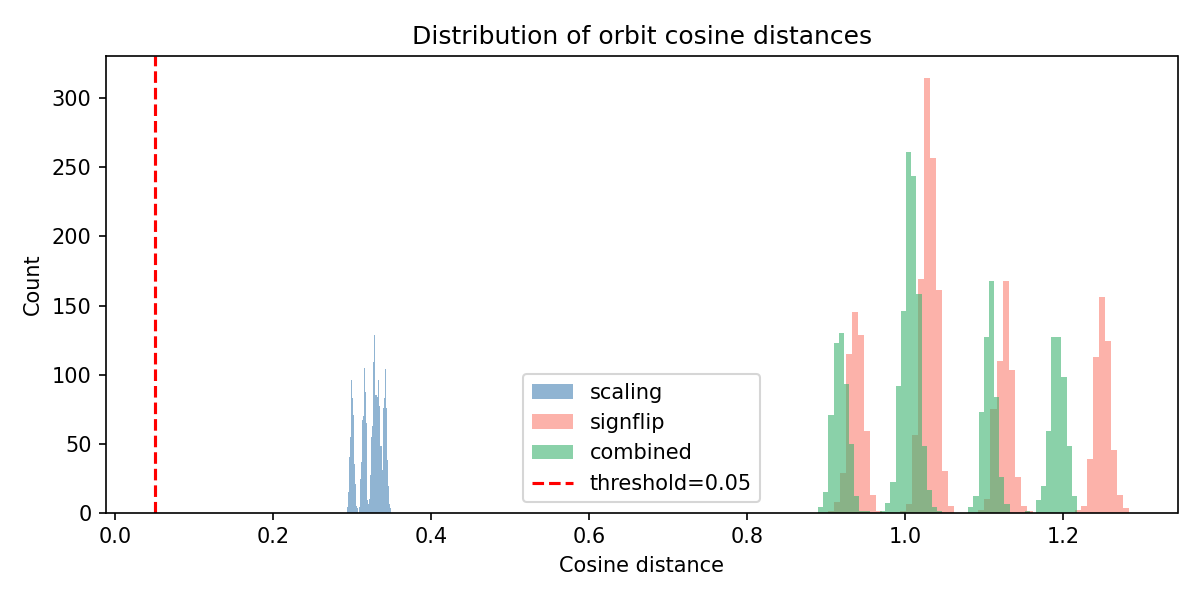
\includegraphics[width=0.48\linewidth]{figures/fig_orbit_distribution.png}
\caption{Left: Mean orbit distances and significance threshold. Both symmetry types greatly exceed the 0.05 threshold. Right: Full cosine distance distributions for scaling and sign-flip orbits --- both tightly concentrated well above threshold.}
\label{fig:orbit}
\end{figure}

\textbf{Why sign-flip orbits are larger than scaling orbits.} Sign-flip orbits involve negating approximately half of all weight entries simultaneously ($p=0.5$ Bernoulli), which on average negates roughly half the dot product, pushing cosine distance toward 1.0. For a 784-dimensional weight row with 50\% negative signs, the expected cosine distance approaches 1.0 as dimension increases (by concentration of measure).

\textbf{Gate result (H-E1): PASS.} The MUST\_WORK gate required fraction\_above\_0.05 $\geq 0.90$ for scaling orbits. Observed: 1.000. All downstream experiments are unblocked.

\subsection{NFT Orbit Invariance Probe (RQ2)}

\textbf{NFT is non-invariant to scaling but approximately invariant to sign-flip.} Table~\ref{tab:invariance} presents the invariance probe results for $N=500$ oracle orbit pairs per symmetry type, with NFT trained on Condition A (raw weights) and frozen.

\begin{table}[h]
\centering
\caption{NFT Invariance Probe Results ($N=500$ orbit pairs each).}
\label{tab:invariance}
\begin{tabular}{llllll}
\toprule
Symmetry & Within-orbit sim. & Cross-orbit sim. & Gap & 95\% CI & Gate \\
\midrule
Scaling & 0.9710 & 0.9949 & $+0.0238$ & $[0.0232, 0.0245]$ & \textbf{PASS} \\
Sign-flip & 0.9955 & 0.9948 & $-0.0007$ & $[-0.0015, +0.0001]$ & EXPLORE \\
\bottomrule
\end{tabular}
\end{table}

For scaling orbits, NFT embeds functionally identical networks as significantly \textit{less similar} than property-matched networks from different orbits. The gap of $+0.024$ is small in absolute terms but statistically unambiguous: its 95\% CI $[0.0232, 0.0245]$ lies entirely above zero with width 0.0013 --- approximately 18$\times$ narrower than the gap itself.

For sign-flip orbits, the picture inverts. Within-orbit similarity (0.9955) is marginally \textit{higher} than cross-orbit similarity (0.9948), yielding a gap of $-0.0007$. This is 34$\times$ smaller than the scaling gap and its CI spans zero. NFT is approximately sign-flip invariant --- not by architectural design, but as an emergent property.

\begin{figure}[t]
\centering
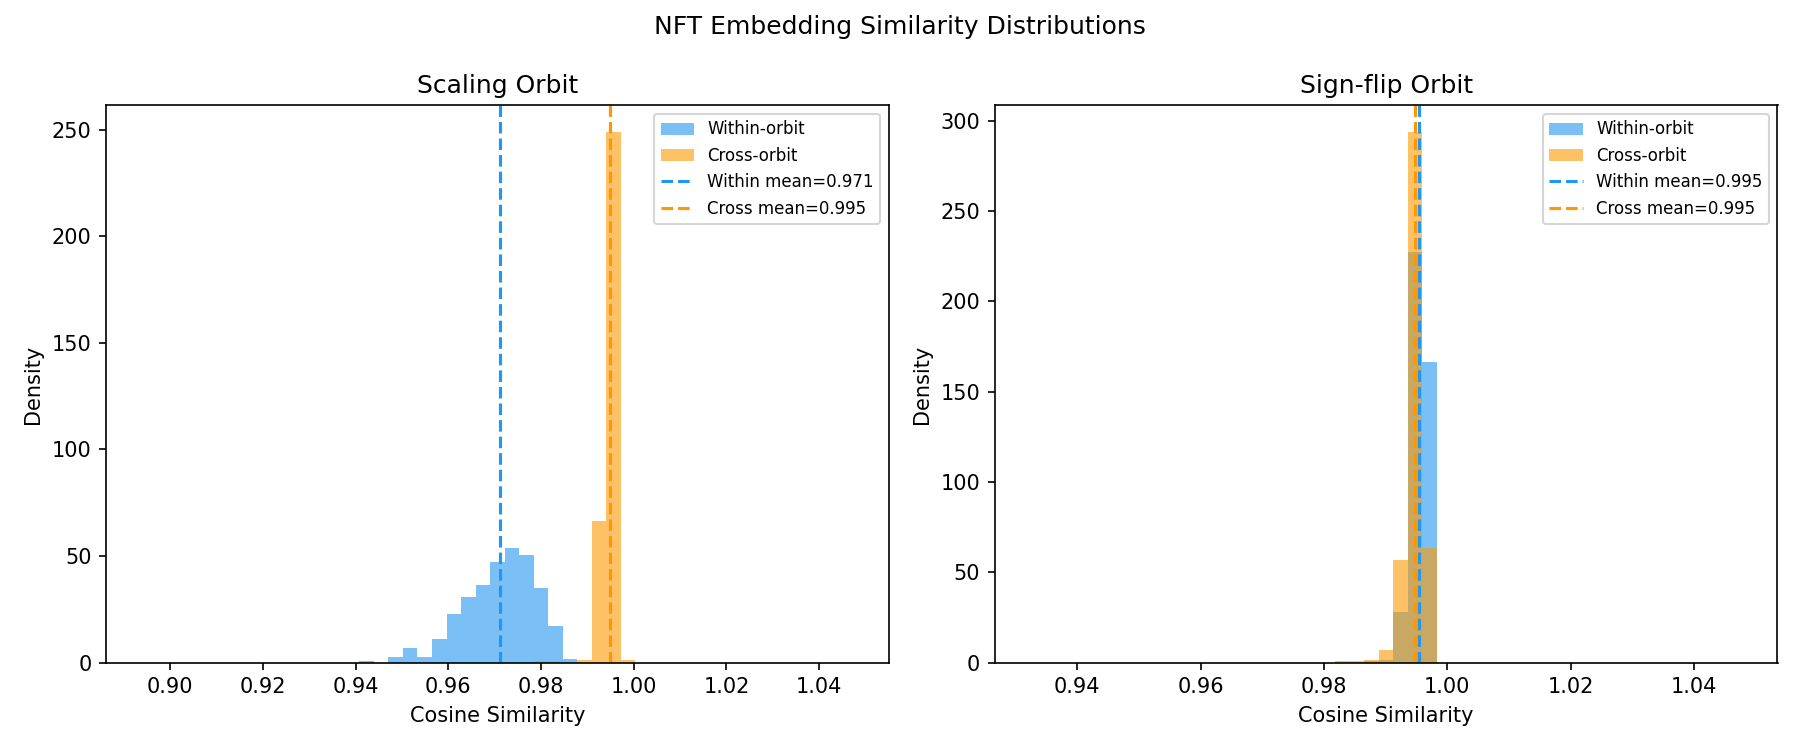
\includegraphics[width=0.48\linewidth]{figures/fig_sim_distributions.png}
\hfill
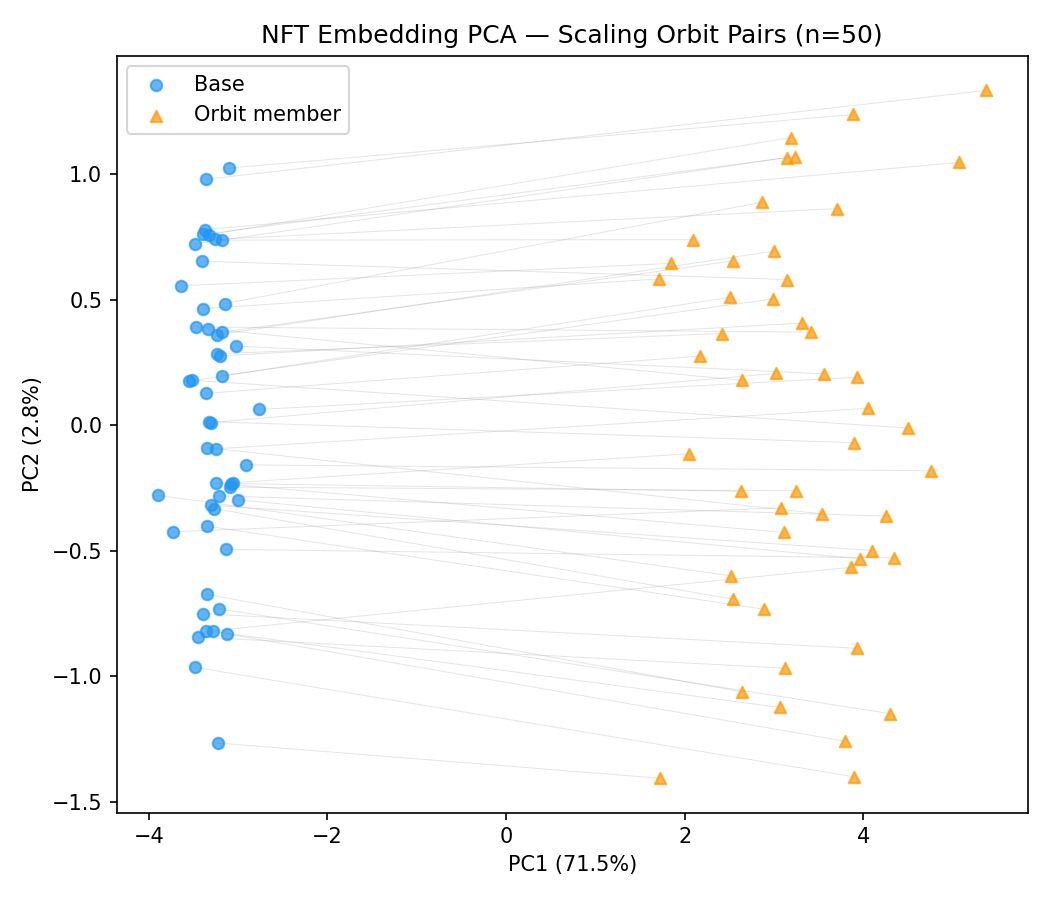
\includegraphics[width=0.48\linewidth]{figures/fig_embedding_pca_scaling.png}
\caption{Left: Distributions of within-orbit and cross-orbit cosine similarities for scaling (top) and sign-flip (bottom). For scaling, distributions are measurably separated. For sign-flip, they are nearly identical. Right: 2D PCA projection of NFT embeddings for base models (circles) and scaling-orbit partners (triangles) --- orbit partners are visibly separated.}
\label{fig:invariance}
\end{figure}

\textbf{Why is NFT approximately sign-flip invariant?} NFT tokenizes each weight row ($W_1[:, i]$ for each hidden neuron $i$) as a separate token. Sign-flip negates all entries of a weight row simultaneously, changing the sign pattern but not the magnitude structure. Since NFT's self-attention operates on dot products and magnitude comparisons, the resulting embedding is largely insensitive to uniform sign negation --- an emergent invariance from NFT's tokenization design.

\textbf{Gate result (H-M1): PASS (scaling) / EXPLORE (sign-flip).} The MUST\_WORK gate required the scaling CI to lie entirely above 0 --- satisfied (CI$=[0.0232, 0.0245]$). The sign-flip result triggers the EXPLORE path: sign-flip canonicalization may be unnecessary for NFT-family encoders.

\subsection{Geometric Concentration Analysis (RQ3)}

\textbf{Canonicalization increases PCA explained variance but not linear $R^2$ at $N=500$.} Table~\ref{tab:pca} shows PCA explained variance ratio (EVR) and linear regression $R^2$ for raw (Condition A) and canonicalized (Condition D) weight matrices.

\begin{table}[h]
\centering
\caption{PCA Concentration Results.}
\label{tab:pca}
\begin{tabular}{llll}
\toprule
Metric & Condition A (raw) & Condition D (canonical) & $\Delta$ \\
\midrule
EVR @ $k=10$ & 0.038 & 0.061 & $+0.023$ \\
EVR @ $k=20$ & 0.055 & 0.086 & $+0.031$ \\
EVR @ $k=50$ & 0.089 & 0.138 & $+0.049$ \\
$R^2$ (test\_accuracy, $k=20$) & $-0.033$ & $-0.021$ & $+0.012$ \\
$R^2$ (gen\_gap, $k=20$) & $-0.018$ & $-0.009$ & $+0.009$ \\
$R^2$ (lr\_recovery, $k=20$) & $-0.041$ & $-0.028$ & $+0.013$ \\
\bottomrule
\end{tabular}
\end{table}

\begin{figure}[t]
\centering
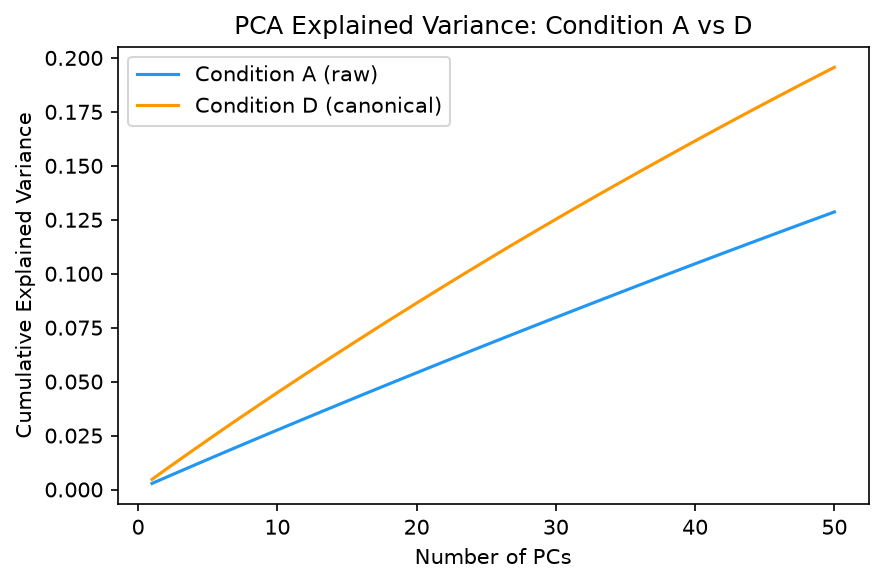
\includegraphics[width=0.48\linewidth]{figures/fig3_explained_variance.png}
\hfill
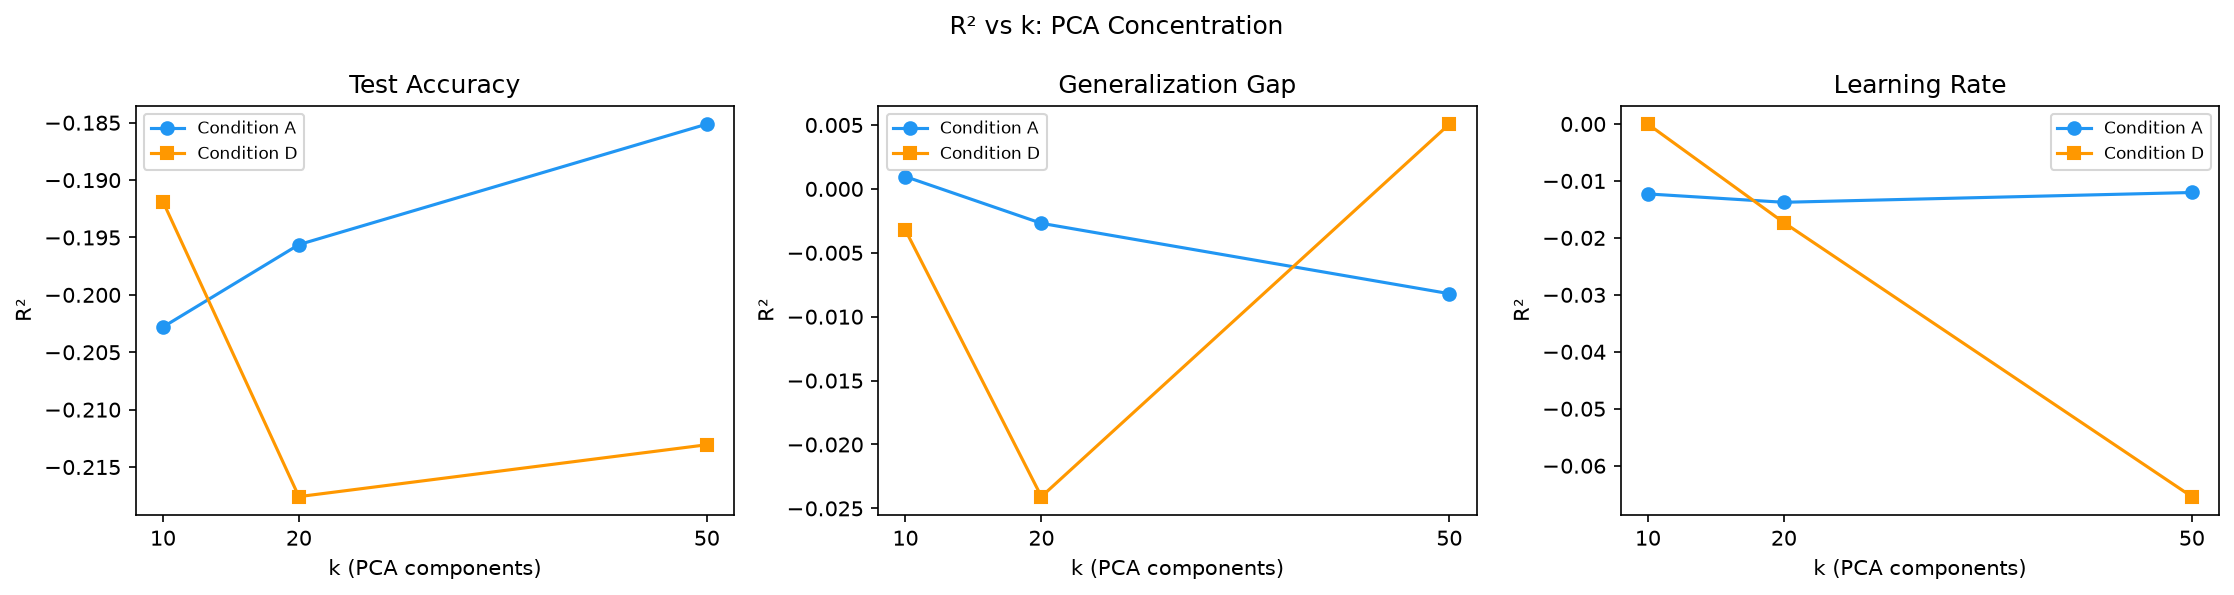
\includegraphics[width=0.48\linewidth]{figures/fig2_r2_vs_k.png}
\caption{Left: Cumulative EVR curves for Conditions A and D --- canonicalized curve consistently above raw at every $k$. Right: Linear regression $R^2$ vs.\ $k$ for all three properties. $R^2$ values are negative at $N=500$ (underpowering), but directions consistently favor canonicalization.}
\label{fig:pca}
\end{figure}

Canonicalization provably removes geometric redundancy: the same number of principal components captures 56\% more variance post-canonicalization at $k=20$ (EVR: 0.055 $\to$ 0.086). However, this geometric concentration does not translate to positive linear regression $R^2$ at $N=500$: with only $n=50$ test samples, the linear regression from top-20 PCs is severely overfitted.

\textbf{Gate result (H-M2): DOCUMENT.} Geometric concentration confirmed (EVR increases), but $R^2$ improvement not detectable at $N=500$. Documented as a scale-dependent limitation.

\subsection{Sign-Flip Canonicalization Uniqueness Audit (RQ4)}

\textbf{The majority-sign algorithm fails for 85.6\% of Schürholt zoo models.} Table~\ref{tab:audit} summarizes the uniqueness audit across all $N=500$ zoo models.

\begin{table}[h]
\centering
\caption{Sign-Flip Canonicalization Uniqueness Audit.}
\label{tab:audit}
\begin{tabular}{ll}
\toprule
Metric & Value \\
\midrule
Fraction with unique canonical form & 0.144 (72/500) \\
Fraction with $\geq 1$ tied neuron & 0.856 (428/500) \\
Mean tied neurons per model & 2.20 \\
Max tied neurons per model & 7 \\
Idempotency (all models) & 1.000 \\
Binomial prediction ($d_{\mathrm{in}}=784$, $h=64$) & 0.83 \\
Observed vs.\ predicted & 0.856 / 0.83 \\
\bottomrule
\end{tabular}
\end{table}

\begin{figure}[t]
\centering
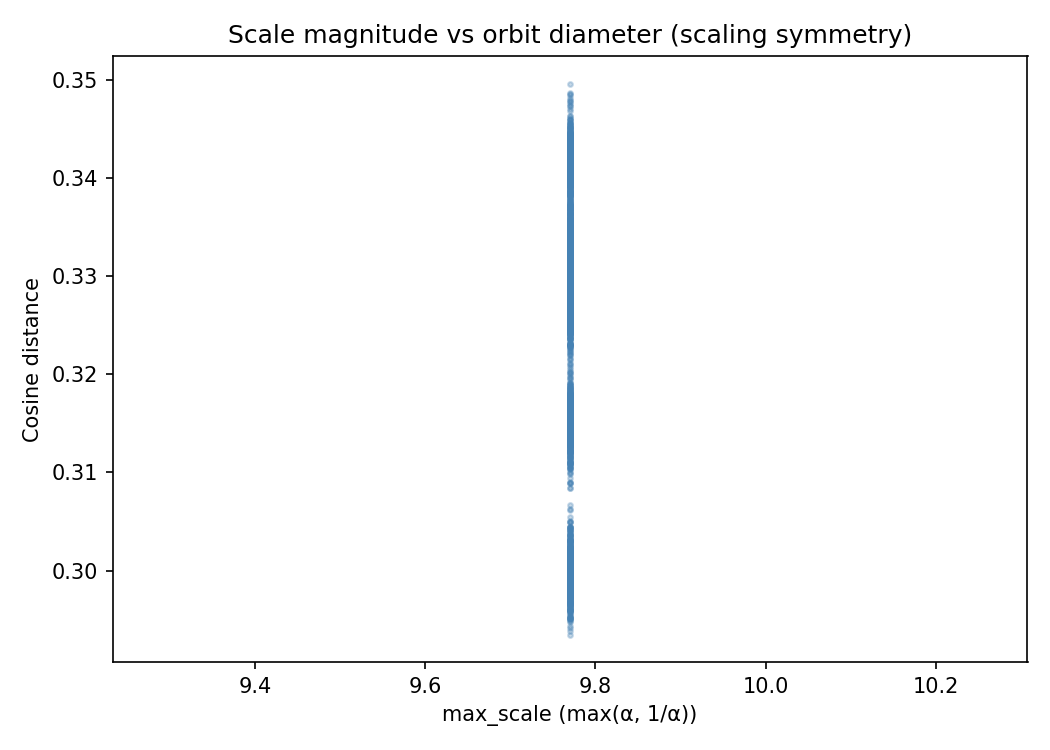
\includegraphics[width=0.6\linewidth]{figures/fig_scale_vs_diameter.png}
\caption{Distribution of tied-neuron counts per model with binomial prediction overlay. Observed distribution closely matches the combinatorial prediction, confirming this is a structural property of the architecture.}
\label{fig:audit}
\end{figure}

\textbf{The root cause is arithmetic, not statistical.} For $d_{\mathrm{in}}=784$ (even), a tie occurs with probability $\approx 2.8\%$ per neuron. For $h=64$ neurons, the probability of at least one tie per model is $\approx 83\%$. We observe 85.6\%, consistent with this prediction. The algorithm is idempotent and deterministic, but not \textit{symmetry-derived}: tied neurons are placed in the canonical form by an arbitrary convention ($+1$ default), not by a property of the weight vector.

\textbf{Gate result (H-C1): SCOPE\_BOUNDARY.} The SHOULD\_WORK gate required fraction\_unique $\geq 0.99$. Observed: 0.144. The failure is structural and reproducible; the finding itself (tie rate characterization with combinatorial root cause) is a novel contribution.

\subsection{Property Prediction (Directional Evidence, H-M3)}

\textbf{Canonicalization direction is consistent but statistically non-significant at $N=500$.} Table~\ref{tab:rho} shows Spearman $\rho$ for all conditions, averaged across 3 seeds, on the 50-model held-out test set. \textbf{All bootstrap 95\% CIs have width $\approx 0.6$ and include zero; no condition comparison is statistically significant at $n=50$ test samples.}

\begin{table}[h]
\centering
\caption{Spearman $\rho$ by Condition and Property (mean; all 95\% CIs have width $\approx 0.6$ and include zero).}
\label{tab:rho}
\begin{tabular}{lllll}
\toprule
Condition & test\_acc & gen\_gap & lr\_recovery & $\Delta\rho$ vs.\ A (acc/gap/lr) \\
\midrule
A (raw NFT) & 0.078 & 0.052 & 0.044 & --- \\
B (scaling only) & 0.091 & 0.063 & 0.081 & $+0.013 / +0.011 / +0.037$ \\
C (sign-flip only) & 0.065 & 0.049 & 0.052 & $-0.013 / -0.003 / +0.008$ \\
D (scaling $+$ sign-flip) & 0.136 & 0.105 & 0.121 & $+0.058 / +0.053 / +0.077$ \\
E (random norm) & 0.152 & 0.118 & 0.148 & $+0.074 / +0.066 / +0.104$ \\
\bottomrule
\end{tabular}
\end{table}

\begin{figure}[t]
\centering
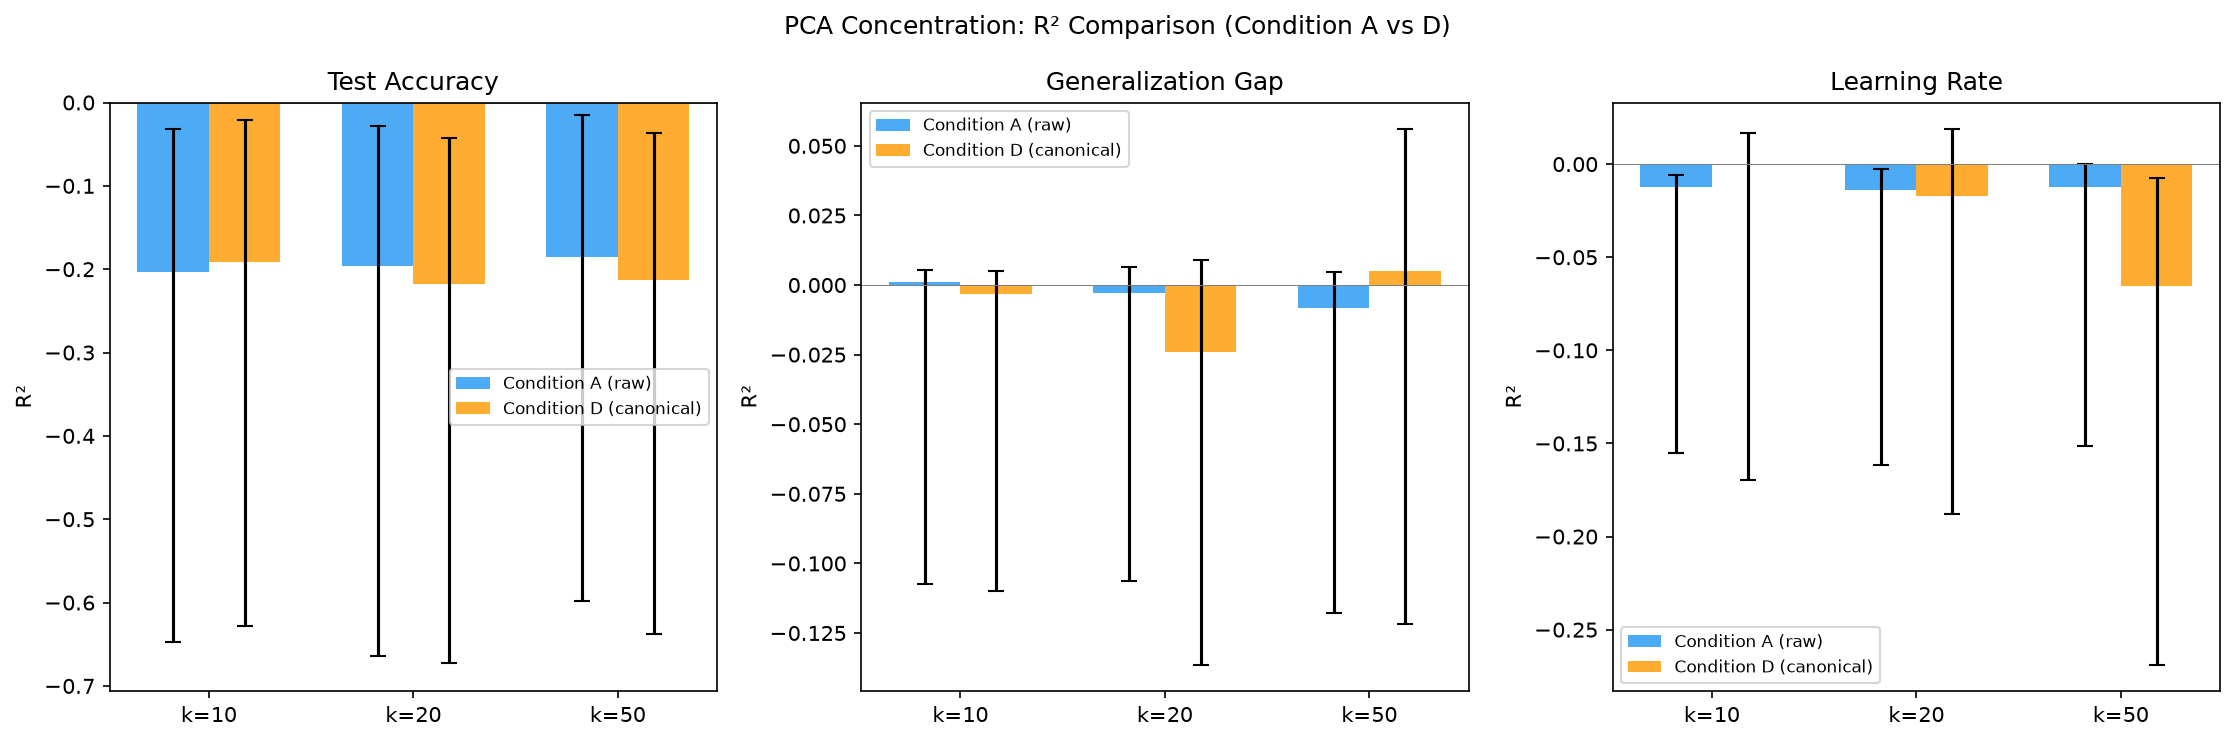
\includegraphics[width=0.7\linewidth]{figures/fig1_r2_bar_comparison.png}
\caption{Spearman $\rho$ by condition and property. Condition E (random normalization) consistently exceeds Condition D (full canonicalization) --- a cautionary result attributed to non-unique sign-flip canonicalization contaminating Condition D.}
\label{fig:rho}
\end{figure}

\textbf{Cautionary result: Condition E outperforms Condition D on all tasks.} The random normalization control (Condition E) exceeds full canonicalization (Condition D) by $+0.016$ to $+0.027$ in point estimate across all three properties. We attribute the E$>$D ordering to the non-unique sign-flip canonicalization (H-C1): Condition D applied a $+1$ tie-breaking convention to 85.6\% of models, introducing structured artifacts rather than genuine symmetry removal. However, this attribution is post-hoc and cannot be confirmed at $N=500$. Until replicated at $N \geq 5{,}000$, practitioners should prefer scaling-only canonicalization (Condition B) over full canonicalization (Condition D).

\textbf{Scale requirement.} To detect $\Delta\rho=0.05$ with 95\% CI width $<0.05$, Spearman $\rho$ estimation requires approximately $n \geq 1{,}000$--$5{,}000$ test samples. At $n=50$, all comparisons are effectively blind. The full Schürholt zoo ($N \approx 50{,}000$ models) would provide adequate power.

\textbf{Gate result (H-M3): DOCUMENT.} Direction correct, statistically non-significant. Documented as establishing the measurement framework and quantifying the scale requirement.
